\chapter{Implementação}
\label{ch:implementation}

Nesse capítulo serão explicadas as particularidades de cada implementacão das funcões mencionadas no capítulo anterior. Também serão elucidados alguns aspectos exclusivos da linguagem Rust, primeiramente abordando algumas decisões de arquitetura e em seguida falando sobre as 3 estruturas de dados implementadas.

\section{Arquitetura}

Como já citado no capítulos anterior, dado que haveriam implementações de funções em comum para estruturas de dados diferentes, grafo e dígrafo foram implementados através de \texttt{traits}, da seguinte forma:

\begin{lstlisting}[language=Java, caption={Implementação do trait Graph}, label=list:trait_graph]
pub trait Graph<Node: Eq + Hash + Copy> {
    fn new_empty() -> Self;

    fn order(&self) -> usize;

    fn size(&self) -> usize;

    fn node_degrees(&self, n: Node) -> (usize, usize);

    fn nodes(&self) -> impl Iterator<Item = Node>;

    fn add_node(&mut self, n: Node);

    fn remove_node(&mut self, n: Node);

    fn add_edge(&mut self, n: Node, m: Node);

    fn remove_edge(&mut self, n: Node, m: Node);

    type Neighbors<'a>: Iterator<Item = Node>
    where
        Self: 'a,
        Node: 'a;
    fn neighbors<'a>(&'a self, n: Node) -> Self::Neighbors<'a>;

    fn biparted(&self) -> bool;

    fn underlying_graph(&self) -> Self;

    fn has_edge(&self, n: Node, m: Node) -> bool {
        self.neighbors(n).any(|neighbor| neighbor == m)
    }

    fn dfs(&self, start: Node) -> DfsIter<'_, Node, Self>
    where
        Self: Sized,
    {
        DfsIter::new(self, start)
    }

    fn bfs(&self, start: Node) -> BfsIter<'_, Node, Self>
    where
        Self: Sized,
    {
        BfsIter::new(self, start)
    }

    fn classify_edges(&self, start: Node) -> DfsEdgesIter<'_, Node, Self>
    where
        Self: Sized,
    {
        DfsEdgesIter::new(self, start)
    }
}
\end{lstlisting}

As particularidades da sintaxe acima são que, \texttt{Graph} pode ser implementado para qualquer tipo genérico \texttt{N}, desde que este implemente os seguintes \textt{traits}:

\begin{itemize}
  \item \textbf{Eq}: Que dá ao tipo a propriedade de igualdade através do operador ==
  \item \textbf{Hash}: Propriedade necessária para que aquele tipo possa ser usado em estruturas de dados como \texttt{HashMap/HashSet}. Que serão usadas em trabalhos futuros.
  \item \textbf{Copy}: Que dá ao tipo a propriedade de ser copiável através do operador =, o que apesar de parecer trivial, não é. E isso acontece pois Rust introduz o conceito de \cite{ownership}, que faz com que nem todo tipo seja copiável.
\end{itemize}

Feito isso, basta com que o tipo implementa as funções com as assinaturas solicitadas e ele terá o \texttt{trait Graph}. E além dele, também temos outro \texttt{trait} que tem ele como pré-requisito para implementação, o \texttt{UndirectedGraph}:

\begin{lstlisting}[language=Java, caption={Implementação do trait UndirectedGraph}, label=list:trait_undirected_graph]
pub trait UndirectedGraph<Node: Copy + Eq + Hash>: Graph<Node> {
    fn undirected_size(&self) -> usize;

    fn connected(&self) -> bool;

    fn biconnected_components(&self, start: Node) -> BiconnectedComponentsIter<'_, Node, Self>
    where
        Self: Sized,
    {
        BiconnectedComponentsIter::new(self, start)
    }

    fn add_undirected_edge(&mut self, n: Node, m: Node) {
        self.add_edge(n, m);
        self.add_edge(m, n);
    }

    fn remove_undirected_edge(&mut self, n: Node, m: Node) {
        self.remove_edge(n, m);
        self.remove_edge(m, n);
    }

    fn undirected_node_degree(&self, n: Node) -> usize {
        self.neighbors(n).count()
    }

    fn classify_undirected_edges<'a>(&'a self, start: Node) -> impl Iterator<Item = Edge<Node>>
    where
        Self: Sized,
        Node: 'a,
    {
        DfsEdgesIter::new(self, start)
            .filter(|edge| matches!(edge, Edge::Tree(_, _) | Edge::Back(_, _)))
    }
}
\end{lstlisting}

Note que o \texttt{trait} já tem várias implementações, e isso só é possível pois ele usa as funcões já implementadas em \textt{Graph}. Por isso que implementar \textt{UndirectedGraph}, antes, é necessário implementar esse.

Mas feitas as considerações iniciais acerca da arquitetura da implementação, podemos abordar as particularidades de cada Estrutura da Dados.

\section{Matriz de Adjacência}

A Matriz de Adjacência, conforme falado anteriormente, é uma das formas mais comuns de se implementar um grafo. Muito disso em decorrência de sua baixa complexidade na inserção e no acesso nos elementos. Sendo assim, ela é implementada da seguinte forma:

\begin{lstlisting}[language=Java, caption={Implementação da Estrutura de Dados Matriz de Adjacência}, label=list:struct_adj_mat]
#[derive(Debug, Clone)]
pub struct AdjacencyMatrix(pub Vec<Vec<usize>>);
\end{lstlisting}

No código acima, o \texttt{derive} é uma instrução para o compilador inferir como adicionar as pripriedades \texttt{Debug} e \texttt{Clone} na estrutura abaixo. Estrutura essa que consiste em um vetor de vetores de \texttt{usize}(inteiros não-negativos, tipo usado para fins de simplificação, uma vez que temos mais garantias sobre as propridades dele dessa forma, diferente de em tipos genéricos). E abaixo segue a implementação das funções solicitadas pelo \texttt{trait UndirectedGraph}.

\begin{lstlisting}[language=Java, caption={Implementação de UndirectedGraph na Estrutura de Dados Matriz de Adjacência}, label=list:impl_adj_mat_ug] impl UndirectedGraph<usize> for AdjacencyMatrix {
    fn undirected_size(&self) -> usize {
        let mut size = 0;
        for i in 0..self.order() {
            for j in 0..=i {
                if self.0[i][j] > 0 {
                    size += 1;
                }
            }
        }
        size
    }

    fn connected(&self) -> bool {
        let n = self.order();
        if n == 0 {
            return true;
        }

        let mut visited = vec![false; n];
        let mut stack = vec![0];
        visited[0] = true;

        while let Some(u) = stack.pop() {
            for (v, &is_edge) in self.0[u].iter().enumerate() {
                if is_edge > 0 && !visited[v] {
                    visited[v] = true;
                    stack.push(v);
                }
            }
        }

        visited.into_iter().all(|v| v)
    }

    fn undirected_node_degree(&self, node: usize) -> usize {
        if let Some(row) = self.0.get(node) {
            row.iter().filter(|&&val| val != 0).count()
        } else {
            0
        }
    }
}
\end{lstlisting}

Note que ele só define as funções que não tem implementação padrão. E algo que também importante para se pontuar é que a palavra \texttt{mut}(abreviação de "mutável") é requerida sempre que desejamos alterar o valor da variável em questão, pois devemos fazer isso de forma explícita, e isso acontece por conta do conceito de \cite{ownership}. E abaixo segue a implementação de \texttt{Graph}:

\begin{lstlisting}[language=Java, caption={Implementação de Graph na Estrutura de Dados Matriz de Adjacência}, label=list:impl_adj_mat_g]
impl Graph<usize> for AdjacencyMatrix {
    fn new_empty() -> Self {
        AdjacencyMatrix(vec![])
    }

    fn order(&self) -> usize {
        self.0.len()
    }

    fn size(&self) -> usize {
        self.0
            .iter()
            .enumerate()
            .map(|(i, _)| self.neighbors(i).count())
            .sum()
    }

    fn node_degrees(&self, n: usize) -> (usize, usize) {
        let out_deg = self.0[n].iter().filter(|&&v| v != 0).count();
        let in_deg = self.0.iter().filter(|row| row[n] != 0).count();
        (in_deg, out_deg)
    }

    fn nodes(&self) -> impl Iterator<Item = usize> {
        0..self.order()
    }

    fn add_node(&mut self, _n: usize) {
        self.0.push(Vec::new());
        let new_order = self.order();

        for r in &mut self.0 {
            while r.len() < new_order {
                r.push(0);
            }
        }
    }

    fn remove_node(&mut self, n: usize) {
        if n < self.0.len() {
            self.0.remove(n);
            for row in self.0.iter_mut() {
                for idx in n + 1..row.len() {
                    row[idx - 1] = row[idx];
                }
                row.pop();
            }
        }
    }

    fn add_edge(&mut self, n: usize, m: usize) {
        if let Some(edges) = self.0.get_mut(n)
            && let Some(edge) = edges.get_mut(m)
        {
            if *edge == 1 {
                return;
            }
            *edge = 1;
        }
    }

    fn remove_edge(&mut self, n: usize, m: usize) {
        if let Some(edges) = self.0.get_mut(n)
            && let Some(edge) = edges.get_mut(m)
        {
            *edge = 0;
        }
    }

    type Neighbors<'a> = std::iter::FilterMap<
        std::iter::Enumerate<std::slice::Iter<'a, usize>>,
        fn((usize, &'a usize)) -> Option<usize>,
    >;

    fn neighbors<'a>(&'a self, n: usize) -> Self::Neighbors<'a> {
        fn filter_fn((i, &weight): (usize, &usize)) -> Option<usize> {
            if weight != 0 { Some(i) } else { None }
        }
        match self.0.get(n) {
            Some(row) => row.iter().enumerate().filter_map(filter_fn),
            None => [].iter().enumerate().filter_map(filter_fn),
        }
    }

    fn biparted(&self) -> bool {
        let n = self.order();
        if n == 0 {
            return true;
        }

        let mut side = vec![None; n]; // None = uncolored, Some(0/1) = partition
        let mut queue = std::collections::VecDeque::new();

        for start in 0..n {
            // skip already colored components
            if side[start].is_some() {
                continue;
            }

            side[start] = Some(0);
            queue.push_back(start);

            while let Some(u) = queue.pop_front() {
                let u_side = side[u].unwrap();

                for (v, &is_edge) in self.0[u].iter().enumerate() {
                    if is_edge == 0 {
                        continue;
                    }

                    if side[v].is_none() {
                        side[v] = Some(1 - u_side);
                        queue.push_back(v);
                    } else if side[v] == Some(u_side) {
                        return false; // adjacent nodes with same color
                    }
                }
            }
        }

        true
    }

    fn underlying_graph(&self) -> Self {
        let mut matrix: AdjacencyMatrix =
            AdjacencyMatrix(vec![vec![0; self.0.len()]; self.0.len()]);

        for (idx_r, row) in self.0.iter().enumerate() {
            for (idx_c, col) in row.iter().enumerate() {
                if *col == 1 && !matrix.has_edge(idx_c, idx_r) {
                    matrix.add_undirected_edge(idx_r, idx_c);
                }
            }
        }

        matrix
    }
}
\end{lstlisting}

Perceba que funções como \texttt{underlying_graph} recorrem a funções definidas em \texttt{UndirectedGraph}, e isso ocorre pois os \texttt{traits} tem acesso mútuo entre as funções definidas pelos tipos que os implementam.

\section{Lista de Adjacência}

Juntamente com a Matriz de Adjacência, a lista de Adjacência é uma das implementações mais comum usadas para grafos. Sua natureza de tamanho dinâmico é usada principalmente para problemas que envolvem muitos vértices e arestas, sendo assim, sua implementação em Rust se dá da seguinte forma:

\begin{lstlisting}[language=Java, caption={Implementação de Graph na Estrutura de Dados Matriz de Adjacência}, label=list:impl_adj_mat_g]
#[derive(Debug, Clone, Default)]
pub struct AdjacencyList(pub Vec<Vec<usize>>);
\end{lstlisting}

Perceba que é análoga à matriz de adjacência, com exceção do \texttt{Default} que cria um comportamento padrão de instanciar a estrutura através de um vetor vazio. E sua implementação de \texttt{UndirectedGraph} é a seguinte:

\begin{lstlisting}[language=Java, caption={Implementação de Graph na Estrutura de Dados Matriz de Adjacência}, label=list:impl_adj_mat_g]
impl UndirectedGraph<usize> for AdjacencyList {
    fn undirected_size(&self) -> usize {
        let mut self_loops = 0;
        let regular_edges: usize = self
            .0
            .iter()
            .enumerate()
            .map(|(i, _)| {
                self.neighbors(i)
                    .filter(|&n| {
                        let is_self_loop = n == i;
                        self_loops += is_self_loop as usize;
                        !is_self_loop
                    })
                    .count()
            })
            .sum();
        regular_edges / 2 + self_loops
    }

    fn connected(&self) -> bool {
        for i in 0..self.order() {
            if self
                .dfs(i)
                .filter(|event| matches!(event, DfsEvent::Discover(_, _)))
                .count()
                != self.order()
            {
                return false;
            }
        }
        true
    }

    fn undirected_node_degree(&self, node: usize) -> usize {
        self.0
            .get(node)
            .map(|neighbors| neighbors.len())
            .unwrap_or(0)
    }
}
\end{lstlisting}

Perceba que, dada a natureza de continuidade de "valores significativos"(ao contrário da Matriz de Adjacência, que, por vezes, tem várias ocorrências de 0), a Estrutura de Dados em questão é muito iterável. Sendo assim, o conteúdo da maioria das funções consiste na chamada de vários métodos em sequência. E o mesmo se aplica para a implementacão de \texttt{Graph}, que recorer muito pouco a laços:

\begin{lstlisting}[language=Java, caption={Implementação de Graph na Estrutura de Dados Matriz de Adjacência}, label=list:impl_adj_mat_g]
impl Graph<usize> for AdjacencyList {
    fn new_empty() -> Self {
        AdjacencyList(vec![])
    }

    fn order(&self) -> usize {
        self.0.len()
    }

    fn size(&self) -> usize {
        self.0.iter().map(|neighbors| neighbors.len()).sum()
    }

    fn node_degrees(&self, n: usize) -> (usize, usize) {
        let out_deg = self.0.get(n).map_or(0, |neighbors| neighbors.len());
        let in_deg = self
            .0
            .iter()
            .filter(|neighbors| neighbors.contains(&n))
            .count();
        (in_deg, out_deg)
    }

    fn nodes(&self) -> impl Iterator<Item = usize> {
        0..self.order()
    }

    fn add_node(&mut self, _n: usize) {
        self.0.push(Vec::new());
    }

    fn remove_node(&mut self, n: usize) {
        if n < self.0.len() {
            self.0.remove(n);
            for neighbors in self.0.iter_mut() {
                neighbors.retain(|&x| x != n);
                for x in neighbors.iter_mut() {
                    if *x > n {
                        *x -= 1;
                    }
                }
            }
        }
    }

    fn add_edge(&mut self, n: usize, m: usize) {
        if self.0.get(m).is_some()
            && let Some(n_edges) = self.0.get_mut(n)
            && !n_edges.contains(&m)
        {
            n_edges.push(m);
        }
    }

    fn remove_edge(&mut self, n: usize, m: usize) {
        if let Some(edges) = self.0.get_mut(n) {
            edges.retain(|&x| x != m);
        }
    }

    type Neighbors<'a> = std::iter::Copied<std::slice::Iter<'a, usize>>;

    fn neighbors<'a>(&'a self, n: usize) -> Self::Neighbors<'a> {
        match self.0.get(n) {
            Some(edges) => edges.iter().copied(),
            None => [].iter().copied(),
        }
    }

    fn biparted(&self) -> bool {
        let n = self.order();
        if n == 0 {
            return true;
        }

        let mut side = vec![None; n];

        for start in 0..n {
            if side[start].is_some() {
                continue;
            }
            side[start] = Some(0);
            let mut queue = std::collections::VecDeque::new();
            queue.push_back(start);

            while let Some(u) = queue.pop_front() {
                let u_side = side[u].unwrap();
                for v in self.neighbors(u) {
                    if side[v].is_none() {
                        side[v] = Some(1 - u_side);
                        queue.push_back(v);
                    } else if side[v] == Some(u_side) {
                        return false;
                    }
                }
            }
        }

        true
    }

    fn underlying_graph(&self) -> Self {
        let mut list = AdjacencyList(vec![Vec::new(); self.0.len()]);

        for (idx_r, row) in self.0.iter().enumerate() {
            for &col in row.iter() {
                if !list.has_edge(idx_r, col) {
                    list.add_undirected_edge(idx_r, col);
                }
            }
        }
        list
    }
}
\end{lstlisting}

Algo válido de se ressaltar é que o uso de \texttt{Some} e \texttt{None} ocorre pois, por vezes, funções retornam um \texttt{Result} que pode ou não conter um valor válido, e esses são os contrutores do tipo. Sendo assim, a linguagem opta por encapsular dessa forma o resultado de certas funções, ao invés de lançar uma exceção(o que geralmente é feito por outras linguagens).

\sections{Matriz de Incidência}

Por motivos já citados, esta se trata de uma das abordagens menos interessantes.

We mentioned in Chapter~\ref{ch:intro} %[example backward reference
% to a chapter or section.]
that a project report's structure could follow a particular paradigm.
Hence, the organization of a report (effectively the Table of Content
of a report) can vary depending on the type of project you are doing.
Check which of the given examples suit your project. Alternatively,
follow your supervisor's advice.

\section{Examples of the sections of a methodology chapter}
A general report structure is summarised (suggested) in
Table~\ref{tab:gen_template}. Table~\ref{tab:gen_template} describes
that, in general, a typical report structure has three main parts:
(1) front matter, (2) main text, and (3) end matter. %[\textbf{also notice that the preceding sentence is an example of a numbered list
% in a text body}].
The structure of the front matter and end matter will remain the same
for all the undergraduate final year project report. However, the
main text varies as per the project's needs.
\begin{table}[!ht]
  \centering
  \caption{Undergraduate report template structure}
  \label{tab:gen_template}
  \begin{tabular}{llll}
    \toprule
    \multirow{7}{3cm}{Frontmatter}
    & & Title Page & \\
    & & Abstract &    \\
    & & Acknowledgements & \\
    & & Table of Contents &    \\
    & & List of Figures   &    \\
    & & List of Tables    &    \\
    & & List of Abbreviations  &    \\
    & &   &    \\
    \multirow{7}{3cm}{Main text}
    & Chapter 1 & Introduction   &    \\
    & Chapter 2 & Literature Review   &    \\
    & Chapter 3 & Methodology   &    \\
    & Chapter 4 & Results    &    \\
    & Chapter 5 & Discussion and Analysis  &    \\
    & Chapter 6 & Conclusions and Future Work  &    \\
    & Chapter 7 & Refection  &    \\
    & &   &    \\
    \multirow{2}{3cm}{End matter}
    & & References  &    \\
    & & Appendices (Optional)  &    \\
    & & Index (Optional)  &    \\
    \bottomrule
  \end{tabular}
\end{table}

\subsection{Example of a software/Web development main text structure}
\label{subsec:se_chpters}
Notice that the ``methodology'' Chapter of Software/Web development
in Table~\ref{tab:soft_eng_temp} takes a standard software
engineering paradigm (approach). Alternatively, these suggested
sections can be the chapters of their own. Also, notice that
``Chapter 5'' in Table~\ref{tab:soft_eng_temp} is ``Testing and
Validation'' which is different from the general report template
mentioned in Table~\ref{tab:gen_template}. Check with your supervisor
if in doubt.
\begin{table}[!ht]
  \centering
  \caption{Example of a software engineering-type report structure}
  \label{tab:soft_eng_temp}
  \begin{tabular}{lll}
    \toprule
    Chapter 1 & Introduction   &    \\
    Chapter 2 & Literature Review  &    \\
    Chapter 3 & Methodology   &    \\
    &               & Requirements specifications   \\
    &               & Analysis   \\
    &               & Design   \\
    &               & Implementations   \\
    Chapter 4 & Testing and Validation  &    \\
    Chapter 5 & Results and Discussion      &    \\
    Chapter 6 & Conclusions and Future Work  &    \\
    Chapter 7 & Reflection  &    \\
    \bottomrule
  \end{tabular}
\end{table}

\subsection{Example of an algorithm analysis main text structure}
Some project might involve the implementation of a state-of-the-art
algorithm and its performance analysis and comparison with other
algorithms. In that case, the suggestion in Table~\ref{tab:algo_temp}
may suit you the best.
\begin{table}[!ht]
  \centering
  \caption{Example of an algorithm analysis type report structure}
  \label{tab:algo_temp}
  \begin{tabular}{lll}
    \toprule
    Chapter 1 & Introduction  &    \\
    Chapter 2 & Literature Review  &    \\
    Chapter 3 & Methodology   &    \\
    &               & Algorithms descriptions  \\
    &               & Implementations   \\
    &               & Experiments design   \\
    Chapter 4 & Results       &  \\
    Chapter 5 & Discussion and Analysis  &    \\
    Chapter 6 & Conclusion and Future Work  &    \\
    Chapter 7 & Reflection  &    \\
    \bottomrule
  \end{tabular}
\end{table}

\subsection{Example of an application type main text structure}
If you are applying some algorithms/tools/technologies on some
problems/datasets/etc., you may use the methodology section
prescribed in Table~\ref{tab:app_temp}.
\begin{table}[!ht]
  \centering
  \caption{Example of an application type report structure}
  \label{tab:app_temp}
  \begin{tabular}{lll}
    \toprule
    Chapter 1 & Introduction  &    \\
    Chapter 2 & Literature Review  &    \\
    Chapter 3 & Methodology   &    \\
    &               & Problems (tasks) descriptions  \\
    &               & Algorithms/tools/technologies/etc. descriptions  \\
    &               & Implementations   \\
    &               & Experiments design and setup   \\
    Chapter 4 & Results       &  \\
    Chapter 5 & Discussion and Analysis  &    \\
    Chapter 6 & Conclusion and Future Work  &    \\
    Chapter 7 & Reflection  &    \\
    \bottomrule
  \end{tabular}
\end{table}

\subsection{Example of a science lab-type main text structure}
If you are doing a science lab experiment type of project, you may
use the  methodology section suggested in Table~\ref{tab:lab_temp}.
In this kind of project, you may refer to the ``Methodology'' section
as ``Materials and Methods.''
\begin{table}[!ht]
  \centering
  \caption{Example of a science lab experiment-type report structure}
  \label{tab:lab_temp}
  \begin{tabular}{lll}
    \toprule
    Chapter 1 & Introduction  &    \\
    Chapter 2 & Literature Review  &    \\
    Chapter 3 & Materials and Methods   &    \\
    &               & Problems (tasks) description  \\
    &               & Materials \\
    &               & Procedures  \\
    &               & Implementations   \\
    &               & Experiment set-up   \\
    Chapter 4 & Results       &  \\
    Chapter 5 & Discussion and Analysis  &    \\
    Chapter 6 & Conclusion and Future Work  &    \\
    Chapter 7 & Reflection  &    \\
    \bottomrule
  \end{tabular}
\end{table}

\subsection{Ethical considerations}
This section addresses ethical aspects of your project. This may include:
informed consent, describing how participants will be informed about
the study's purpose, procedures, risks, and benefits. You should
detail the process used for obtaining consent and ensuring
participants understand their rights.

\begin{itemize}
  \item \textbf{Informed Consent}: If data was collected from
    participant, detail the process for obtaining consent and
    ensuring participants understand their rights.

  \item \textbf{Confidentiality and Privacy}: Explain measures taken
    to protect participants' data and maintain confidentiality.
    Discuss how data is stored, who will have access, and how
    anonymity will be preserved.

  \item \textbf{Risk Assessment}: Identify potential risks to
    participants and outline strategies to minimize them.

  \item \textbf{Vulnerable Populations}: If applicable, address how
    you will protect vulnerable groups (e.g., children, elderly, or
    marginalized communities) involved in your project.

  \item \textbf{Research Integrity}: Highlight your commitment to
    honesty and transparency in research. Discuss how you will avoid
    plagiarism, fabrication, and falsification of data.

  \item \textbf{Compliance with Regulations}: Mention relevant
    ethical guidelines and regulations that your project will adhere to.

  \item \textbf{Impact on Society}: Reflect on the broader
    implications of your project. Discuss how the outcomes may affect
    communities, stakeholders, or the environment, and how you plan
    to address any potential negative consequences.

  \item \textbf{Feedback Mechanisms}: Describe how you incorporate
    feedback from participants and stakeholders to improve the
    ethical conduct of the project throughout its duration.

\end{itemize}

\section{Example of an Equation in \LaTeX}
Eq.~\ref{eq:eq_example} [note that this is an example of an
equation's in-text citation] is an example of an equation in \LaTeX.
In Eq.~\eqref{eq:eq_example}, $ s $ is the mean of elements $ x_i \in
\mathbf{x} $:

\begin{equation}
  \label{eq:eq_example} % label used to refer the eq in text
  s = \frac{1}{N} \sum_{i = 1}^{N} x_i.
\end{equation}

Have you noticed that all the variables of the equation are defined
using the \textbf{in-text} maths command \$.\$, and
Eq.~\eqref{eq:eq_example} is treated as a part of the sentence with
proper punctuation? Always treat an equation or expression as a part
of the sentence.

\section{Example of a Figure in \LaTeX}
Figure~\ref{fig:chart_a} is an example of a figure in \LaTeX. For
more details, check the link:

\href{https://en.wikibooks.org/wiki/LaTeX/Floats,_Figures_and_Captions}{wikibooks.org/wiki/LaTeX/Floats,\_Figures\_and\_Captions}.

\noindent
Keep your artwork (graphics, figures, illustrations) clean and
readable. At least 300dpi is a good resolution of a PNG format
artwork. However, an SVG format artwork saved as a PDF will produce
the best quality graphics. There are numerous tools out there that
can produce vector graphics and let you save that as an SVG file
and/or as a PDF file. One example of such a tool is the ``Flow
algorithm software''. Here is the link for that:
\href{http://www.flowgorithm.org/download/}{flowgorithm.org}.
\begin{figure}[!ht]
  \centering
  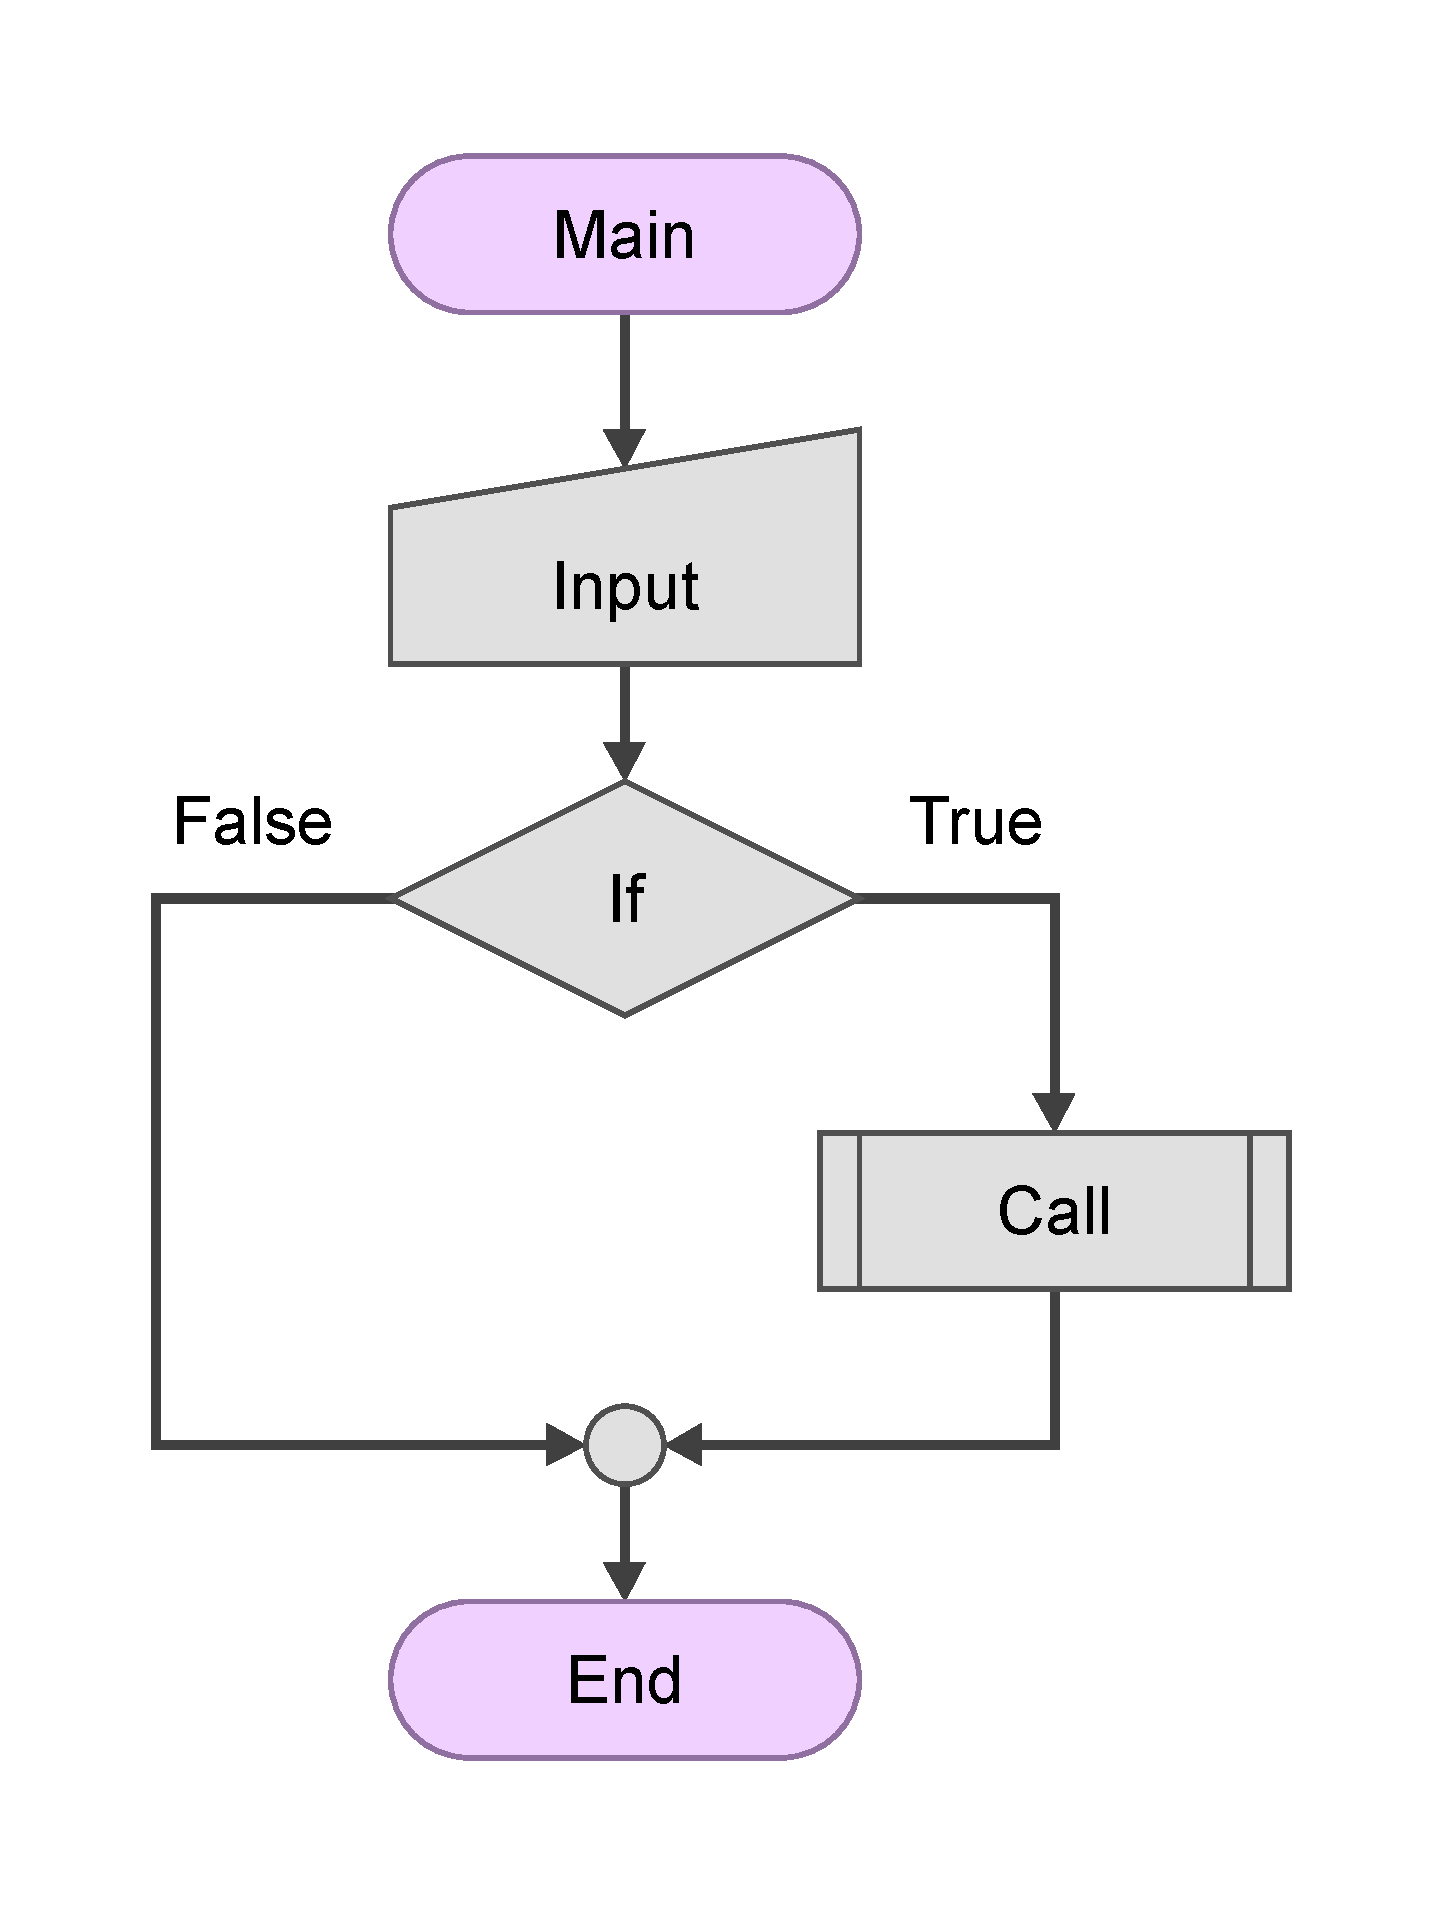
\includegraphics[scale=0.3]{figures/chart.pdf}
  \caption{Example figure in \LaTeX.}
  \label{fig:chart_a}
\end{figure}

\clearpage %  use command \clearpage when you want section or text to
% appear in the next page.

\section{Example of an algorithm in \LaTeX}
Algorithm~\ref{algo:algo_example} is a good example of an algorithm in \LaTeX.
\begin{algorithm}
  \caption{Example caption: sum of all even numbers}
  \label{algo:algo_example}
  \begin{algorithmic}[1]
    \Require{$ \mathbf{x}  = x_1, x_2, \ldots, x_N$}
    \Ensure{$EvenSum$ (Sum of even numbers in $ \mathbf{x} $)}
    \Statex
    \Function{EvenSummation}{$\mathbf{x}$}
    \State {$EvenSum$ $\gets$ {$0$}}
    \State {$N$ $\gets$ {$length(\mathbf{x})$}}
    \For{$i \gets 1$ to $N$}
    \If{$ x_i\mod 2 == 0$}  \Comment Check whether a number is even.
    \State {$EvenSum$ $\gets$ {$EvenSum + x_i$}}
    \EndIf
    \EndFor
    \State \Return {$EvenSum$}
    \EndFunction
  \end{algorithmic}
\end{algorithm}

\section{Example of code snippet  in \LaTeX}

Code Listing~\ref{list:python_code_ex} is a good example of including
a code snippet in a report. While using code snippets, take care of
the following:
\begin{itemize}
  \item do not paste your entire code (implementation) or everything
    you have coded. Add code snippets only.
  \item The algorithm shown in Algorithm~\ref{algo:algo_example} is
    usually preferred over code snippets in a technical/scientific report.
  \item Make sure the entire code snippet or algorithm stays on a
    single page and does not overflow to another page(s).
\end{itemize}

Here are three examples of code snippets for three different
languages (Python, Java, and CPP) illustrated in
Listings~\ref{list:python_code_ex}, \ref{list:java_code_ex}, and
\ref{list:cpp_code_ex} respectively.

\begin{lstlisting}[language=Python, caption={Code snippet in \LaTeX ~and  this is a Python code example}, label=list:python_code_ex]
import numpy as np

x  = [0, 1, 2, 3, 4, 5] # assign values to an array
evenSum = evenSummation(x) # call a function

def evenSummation(x):
    evenSum = 0
    n = len(x)
    for i in range(n):
        if np.mod(x[i],2) == 0: # check if a number is even?
            evenSum = evenSum + x[i]
    return evenSum
\end{lstlisting}

Here we used  the ``\textbackslash clearpage'' command and forced-out
the second listing example onto the next page.
\clearpage  %
\begin{lstlisting}[language=Java, caption={Code snippet in \LaTeX ~and  this is a Java code example}, label=list:java_code_ex]
public class EvenSum{
    public static int evenSummation(int[] x){
        int evenSum = 0;
        int n = x.length;
        for(int i = 0; i < n; i++){
            if(x[i]%2 == 0){ // check if a number is even?
                evenSum = evenSum + x[i];
            }
        }
        return evenSum;
    }
    public static void main(String[] args){
        int[] x  = {0, 1, 2, 3, 4, 5}; // assign values to an array
        int evenSum = evenSummation(x);
        System.out.println(evenSum);
    }
}
\end{lstlisting}

\begin{lstlisting}[language=C, caption={Code snippet in \LaTeX ~and  this is a C/C++ code example}, label=list:cpp_code_ex]
int evenSummation(int x[]){
    int evenSum = 0;
    int n = sizeof(x);
    for(int i = 0; i < n; i++){
        if(x[i]%2 == 0){ // check if a number is even?
            evenSum = evenSum + x[i];
      }
    }
    return evenSum;
}

int main(){
    int x[]  = {0, 1, 2, 3, 4, 5}; // assign values to an array
    int evenSum = evenSummation(x);
    cout<<evenSum;
    return 0;
}
\end{lstlisting}

\section{Example of in-text citation style}
\subsection{Example of the equations and illustrations placement and
reference in the text}
Make sure whenever you refer to the equations, tables, figures,
algorithms,  and listings for the first time, they also appear
(placed) somewhere on the same page or in the following page(s).
Always make sure to refer to the equations, tables and figures used
in the report. Do not leave them without an \textbf{in-text
citation}. You can refer to equations, tables and figures more them once.

\subsection{Example of the equations and illustrations style}
Write \textbf{Eq.} with an uppercase ``Eq`` for an equation before
using an equation number with (\textbackslash eqref\{.\}). Use
``Table'' to refer to a table, ``Figure'' to refer to a figure,
``Algorithm'' to refer to an algorithm and ``Listing'' to refer to
listings (code snippets). Note that, we do not use the articles
``a,'' ``an,'' and ``the'' before the words Eq., Figure, Table, and
Listing, but you may use an article for referring the words figure,
table, etc. in general.

For example, the sentence ``A report structure is shown in
\textbf{the} Table~\ref{tab:gen_template}'' should be written as ``A
report structure is shown \textbf{in} Table~\ref{tab:gen_template}.''

\section{Summary}
Write a summary of this chapter.

~\\[5em]
\noindent
{\huge\textbf{Note:}} In the case of \textbf{software engineering}
project a Chapter ``\textbf{Testing and Validation}'' should precede
the ``Results'' chapter. See Section~\ref{subsec:se_chpters} for
report organization of such project.
